
% Copyright 2004 by Till Tantau <tantau@users.sourceforge.net>.
%
% In principle, this file can be redistributed and/or modified under
% the terms of the GNU Public License, version 2.
%
% However, this file is supposed to be a template to be modified
% for your own needs. For this reason, if you use this file as a
% template and not specifically distribute it as part of a another
% package/program, I grant the extra permission to freely copy and
% modify this file as you see fit and even to delete this copyright
% notice. 

\documentclass[pdf]{beamer}
\mode<presentation>{}

\usepackage[utf8]{inputenc}
\usepackage{amssymb}
\usepackage{amsmath}
\usepackage{graphicx}


% There are many different themes available for Beamer. A comprehensive
% list with examples is given here:
% http://deic.uab.es/~iblanes/beamer_gallery/index_by_theme.html
% You can uncomment the themes below if you would like to use a different
% one:
%\usetheme{AnnArbor}
%\usetheme{Antibes}
%\usetheme{Bergen}
%\usetheme{Berkeley}
%\usetheme{Berlin}
%\usetheme{Boadilla}
%\usetheme{boxes}
%\usetheme{CambridgeUS}
%\usetheme{Copenhagen}
%\usetheme{Darmstadt}
%\usetheme{default}
%\usetheme{Frankfurt}
%\usetheme{Goettingen}
%\usetheme{Hannover}
%\usetheme{Ilmenau}
%\usetheme{JuanLesPins}
%\usetheme{Luebeck}
%\usetheme{Madrid}
%\usetheme{Malmoe}
%\usetheme{Marburg}
%\usetheme{Montpellier}
%\usetheme{PaloAlto}
%\usetheme{Pittsburgh}
%\usetheme{Rochester}
%\usetheme{Singapore}
%\usetheme{Szeged}
\usetheme{Warsaw}



\title{Orthogonal Range Searching in $2$D\\ using Ball Inheritance}
\author{Mads Ravn}
\institute{Computer Science, Aarhus University}
\date{2015}
 
\pgfdeclareimage[height=0.5cm]{university-logo}{logo-eps-converted-to.pdf}
\logo{\pgfuseimage{university-logo}}

% Delete this, if you do not want the table of contents to pop up at
% the beginning of each subsection:
\AtBeginSubsection[]
{
  \begin{frame}<beamer>{Outline}
    \tableofcontents[currentsection,currentsubsection]
  \end{frame}
}

% Let's get started
\begin{document}

\begin{frame}
  \titlepage
\end{frame}

\begin{frame}{Outline}
  \tableofcontents
  % You might wish to add the option [pausesections]
\end{frame}

\section{Introduction}
\subsection{Orthogonal Range Searching}

\begin{frame}{Orthogonal Range Searching}
  \frametitle{Orthogonal Range Searching}
  \begin{center}
    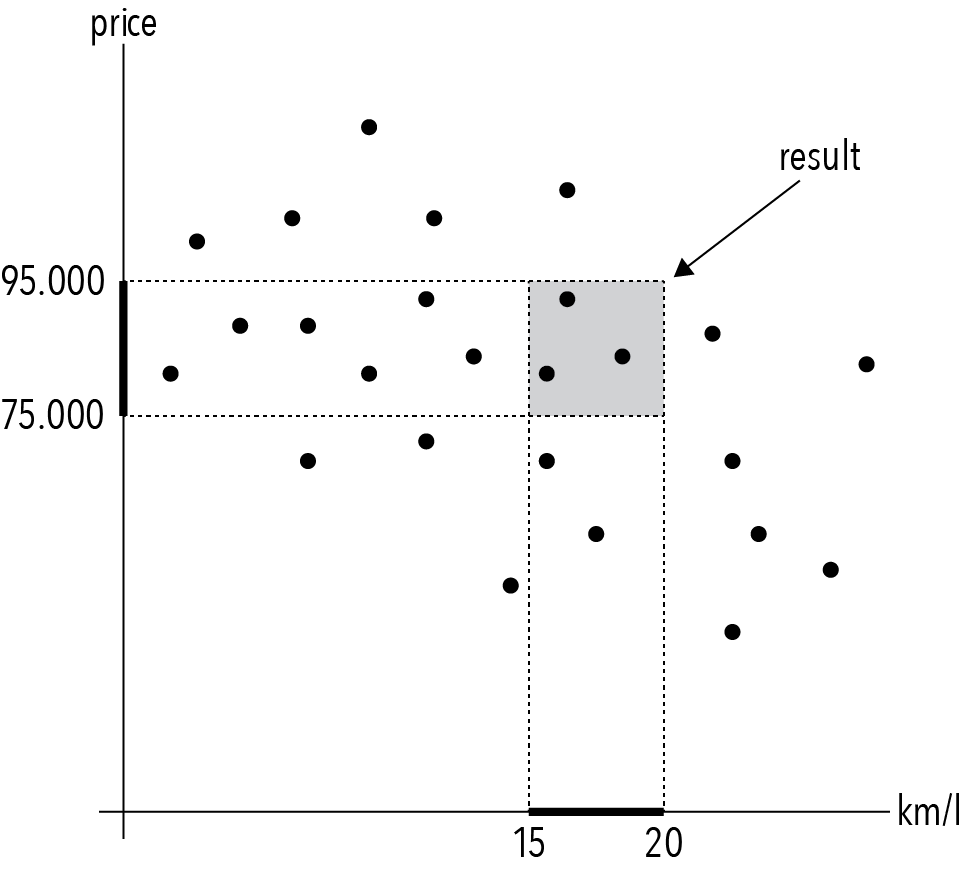
\includegraphics{pictures/introduction.png}
  \end{center}
\end{frame}

\begin{frame}{Preleminaries}
  \frametitle{Preleminaries}
  \begin{itemize}
    \item Alle koordinater er unikke
    \item Rank space
    \item $n$ er en potens af $2$
  \end{itemize}
\end{frame}

\begin{frame}{Orthogonal Range Searching}
  \frametitle{Orthogonal Range Searching}

  Vi er givet $n$ punkter fra $\mathbb{R}^2$ som vi ønsker at indsætte i en datastruktur sådan at vi kan svare effektivt på forespørgslen $q = [x_1, x_2] \times [y_1, y_2]$.
\end{frame}

\subsection{Previous data structures}

\begin{frame}{kd-træ}
  \frametitle{kd-træ}
  \textbf{kd-træ}
  \begin{itemize}
    \item $\mathcal{O}(n)$ plads
    \item $\mathcal{O}(\sqrt{n} + k)$ tid
  \end{itemize}
  Givet $n$ punkter: Punkterne bliver sorteret efter $x$ eller $y$ på skift. Median bliver fundet og punkterne mindre end medianen bliver givet til venstre barn og punkterne højere end medianen bliver givet til højre barn. Et punkt per blad i træet.
\end{frame}

\begin{frame}{Opbygning}
  \frametitle{Opbygning af kd-træ}
  Det $\lceil \frac{n}{2} \rceil$'te element bliver valgt som median. Dette element fungerer som en skille-linje mellem de to punkt-mængder. Medianen bliver låst fast på denne plads i arrayet.
  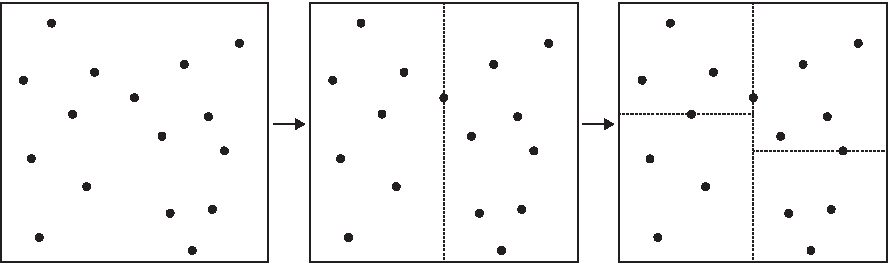
\includegraphics[scale=0.75]{pictures/kd_subdivision-eps-converted-to.pdf}
\end{frame}


\begin{frame}{Søgning}
  \frametitle{Søgning i kd-træ}
  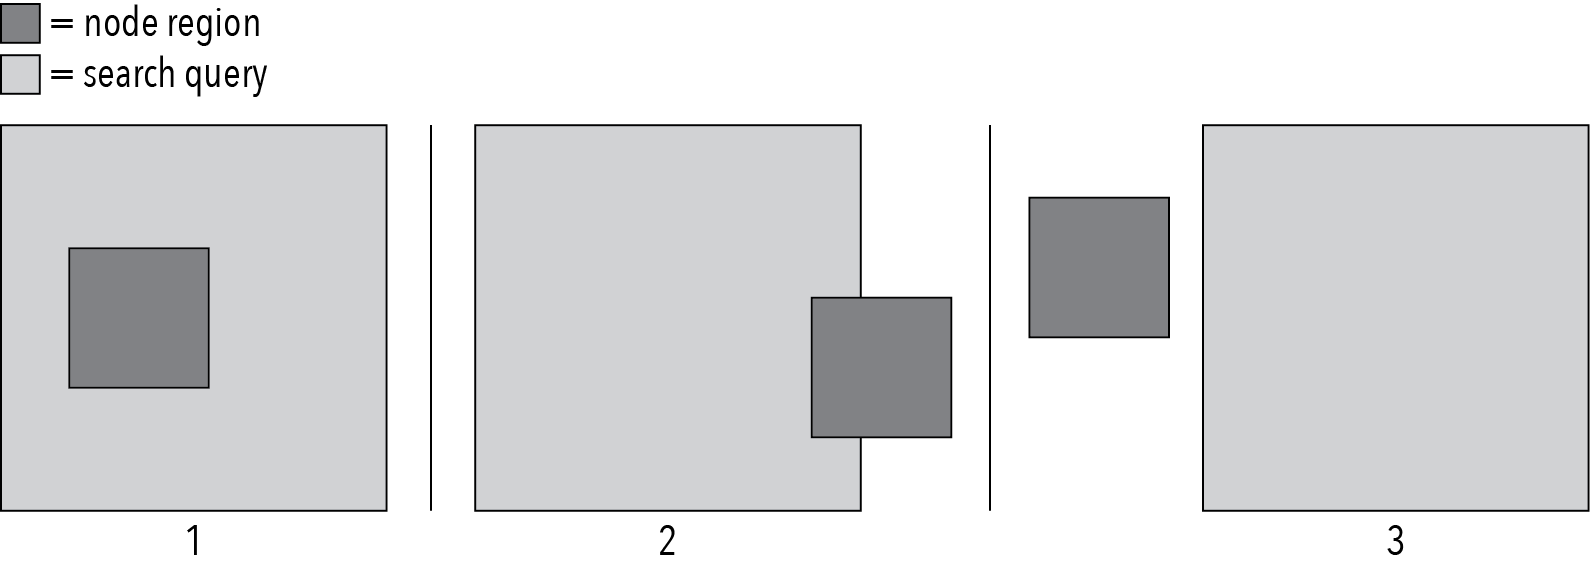
\includegraphics[scale=0.75]{pictures/search_query_overlap.png}
\end{frame}


% Section and subsections will appear in the presentation overview
% and table of contents.

\subsection{First Subsection}

\begin{frame}{First Slide Title}{Optional Subtitle}
  \begin{itemize}
  \item {
    My first point.
  }
  \item {
    My second point.
  }
  \end{itemize}
\end{frame}

\subsection{Ball Inheritance}

% You can reveal the parts of a slide one at a time
% with the \pause command:
\begin{frame}{Ball Inheritance}
  Given a perfect balanced binary tree, each ball include a list of the balls passing through. Consider each ball to have $\lg n$ copies - one for each level in the tree.
\end{frame}

\section{Second Main Section}

\subsection{Another Subsection}

\begin{frame}{Blocks}
\begin{block}{Block Title}
You can also highlight sections of your presentation in a block, with it's own title
\end{block}
\begin{theorem}
There are separate environments for theorems, examples, definitions and proofs.
\end{theorem}
\begin{example}
Here is an example of an example block.
\end{example}
\end{frame}

% Placing a * after \section means it will not show in the
% outline or table of contents.
\section*{Summary}

\begin{frame}{Summary}
  \begin{itemize}
  \item
    The \alert{first main message} of your talk in one or two lines.
  \item
    The \alert{second main message} of your talk in one or two lines.
  \item
    Perhaps a \alert{third message}, but not more than that.
  \end{itemize}
  
  \begin{itemize}
  \item
    Outlook
    \begin{itemize}
    \item
      Something you haven't solved.
    \item
      Something else you haven't solved.
    \end{itemize}
  \end{itemize}
\end{frame}



% All of the following is optional and typically not needed. 
\appendix
\section<presentation>*{\appendixname}
\subsection<presentation>*{For Further Reading}

\begin{frame}[allowframebreaks]
  \frametitle<presentation>{For Further Reading}
    
  \begin{thebibliography}{10}
    
  \beamertemplatebookbibitems
  % Start with overview books.

  \bibitem{Author1990}
    A.~Author.
    \newblock {\em Handbook of Everything}.
    \newblock Some Press, 1990.
 
    
  \beamertemplatearticlebibitems
  % Followed by interesting articles. Keep the list short. 

  \bibitem{Someone2000}
    S.~Someone.
    \newblock On this and that.
    \newblock {\em Journal of This and That}, 2(1):50--100,
    2000.
  \end{thebibliography}
\end{frame}

\end{document}


